\documentclass[conference]{IEEEtran}
\usepackage{amsmath,amssymb,graphicx,booktabs,array,url}
\usepackage[hidelinks]{hyperref}
\usepackage{tikz}
\usetikzlibrary{arrows.meta,positioning}
\newcommand{\statusnote}[1]{\par\smallskip\noindent\textbf{Status:} #1\par\smallskip}
\newcommand{\evidencefigure}[2]{\IfFileExists{generated/#1}{\begin{figure}[!ht]\centering\includegraphics[width=\linewidth,height=.66\textheight,keepaspectratio]{generated/#1}\caption{#2}\end{figure}}{}}
\title{Image Restoration with Universal and Routed Autoencoders\\and Style-Conditioned Face-to-Sketch Generation}
\author{\IEEEauthorblockN{Muhammad Abdullah Masood}\IEEEauthorblockA{23I-0756\\Generative AI}}
\begin{document}
\maketitle
\begin{abstract}
This project implements four connected generative imaging workflows: a universal
denoising autoencoder, a hard-routed system of specialist autoencoders, a jointly
trained soft mixture, and a style-conditioned paired conditional GAN. The first
three share the Oxford-IIIT Pet split and corruption definitions; the fourth
uses paired FS2K photographs and sketches. The implementation uses
validation-only selection of hyperparameters and checkpoints, with final model hashes frozen before test evaluation (Section~\ref{sec:protocol}) and deploys
verified ONNX inference through a React and FastAPI application started with
Docker Compose. The following sections report the recorded final test measurements. On 36,690 deterministic test inputs the corruption classifier reaches 96.8\% accuracy (macro F1 0.950). Predicted routing changes mean PSNR by +9.6 dB on salt-and-pepper noise and +8.2 dB on occlusion, but by -1.7 dB on blur, where the soft mixture reaches -0.4 dB. The sketch generator reaches a mean SSIM of 0.45 and produces smooth sketches without stroke detail.
\end{abstract}
\begin{IEEEkeywords}denoising autoencoder, mixture of experts, conditional GAN, ONNX\end{IEEEkeywords}

\section{Introduction}
Image restoration reconstructs a clean target when the observed image is
affected by impulse noise, blur, or missing regions. A universal model offers a
single reconstruction path, while specialist models can allocate capacity to
individual corruption types. Hard routing introduces classifier mistakes; soft
routing permits uncertain inputs to combine several outputs. Paired sketch
generation additionally requires a style condition and an adversarial objective.
The research questions are whether specialization improves reconstruction,
how routing errors change quality, whether soft weights remain balanced, and
whether a compact conditional generator responds to the three FS2K styles.
These questions require measured results rather than assumed rankings.
The contributions are: (i) a runtime-corruption pipeline with deterministic
validation and test manifests; (ii) a compressed universal autoencoder, a
classifier-routed set of specialists, and a jointly trained soft mixture that
share one data protocol; (iii) a style-conditioned paired GAN; (iv) Optuna and
MLflow records for every task; and (v) one Docker Compose application exposing
all four workspaces through verified ONNX models.

\section{Related Research and Design Alternatives}
Autoencoders learn compact representations by forcing data through a
bottleneck \cite{hinton}, and denoising training maps corrupted inputs to clean
targets \cite{vincent}. Supervised convolutional restoration networks such as
DnCNN \cite{dncnn} and encoder-decoder networks with long skip connections such
as U-Net \cite{unet} are strong baselines. Skip connections were deliberately
not used in the restoration autoencoders: they would let the decoder copy
uncompressed input features, which the assignment's bottleneck requirement
excludes. The consequence, examined in Section~\ref{sec:discussion}, is limited
texture recovery.

SSIM evaluates local structural agreement \cite{wang}; L1 penalizes pixel
differences. Combining them provides distinct reconstruction signals, but their
weight is selected through validation. The soft system follows the mixture-of-experts
idea of Jacobs et al.\ \cite{jacobs}. Expert imbalance is a known concern
\cite{shazeer,switch}; this project uses a dense output mixture with the
assignment's batch-mean balance penalty, not the sparse routing of those works.
Conditional GANs \cite{gan,cgan} and paired translation with a U-Net generator
and local (PatchGAN) discriminator \cite{isola} motivate Task~4, using FS2K
\cite{fs2kpaper}. The compact discriminator here has a 38-pixel receptive
field; it is a local discriminator variant rather than the original 70-pixel design.

\begin{table}[!ht]\centering\caption{Alternatives investigated and the decision taken}\scriptsize
\renewcommand{\arraystretch}{1.12}\begin{tabular}{>{\raggedright\arraybackslash}p{.25\linewidth}>{\raggedright\arraybackslash}p{.36\linewidth}>{\raggedright\arraybackslash}p{.24\linewidth}}\toprule
Alternative & Evidence or reasoning & Decision\\\midrule
Restoration U-Net with long skips & Bypasses the required bottleneck \cite{unet} & Rejected\\
Dense latent vector (128 values) & Collapsed, nearly constant outputs in validation grids (objective 0.322) & Replaced by spatial latent\\
$8{\times}8$ spatial latent (512 values) & Objective 0.281; coarse shapes, large colour error & Replaced by $16{\times}16$\\
GroupNorm in the autoencoder & Per-input statistics; BatchNorm \cite{batchnorm} with tracked statistics tested next & BatchNorm adopted\\
Learning rate $10^{-3}$ & Saturated outputs in a pilot & Rejected; $\le 5{\times}10^{-4}$ searched\\
Bilinear resize + conv & Compared with PixelShuffle decoder \cite{shi} & PixelShuffle + ICNR \cite{aitken}\\
Sparse top-$k$ gating \cite{shazeer} & Only three experts; dense blend is differentiable and matches the brief & Dense softmax gate\\
Per-batch entropy regulariser \cite{switch} & Not evaluated; assignment's squared deviation kept & Squared deviation from $1/4$\\\bottomrule
\end{tabular}\end{table}
The pilot objectives in the table are the validation measurements recorded
in Section~\ref{sec:discussion} and the project's research notes; they are
exploratory sequential changes rather than controlled single-factor ablations.

\section{Data Preparation and Reproducibility}
All images are RGB and resized to $128\times128$ with bicubic interpolation.
The Oxford official trainval membership \cite{pets} is split with NumPy random seed 42,
yielding 2,944 training and 736 validation images. The official test set contains
3,669 images. The same membership is used for Tasks 1--3; breed labels do not
supervise restoration. Source archives and preparation code are retained with
manifest hashes. Test images are downloaded and resized during preparation,
but never loaded by training or hyperparameter selection.

The official FS2K annotations define 1,058 development pairs and 1,046 test
pairs \cite{fs2k}. A stratified 15\% validation split with seed 42 yields 899
training and 159 validation pairs. Training style counts are 303/298/298 and
validation counts are 54/52/53. Style labels are read from annotations, not
inferred from folder names. The official photograph-to-sketch filename mapping
is preserved. Horizontal flips are applied identically to both images in a
training pair.

\subsection{Runtime Corruptions}
Every clean training image receives a freshly sampled condition. The universal
model samples each of four conditions with equal probability; classifier and
gate batches enforce equal counts. Salt-and-pepper probability is uniform in
$[0.02,0.15]$, with selected RGB pixels set to black or white equiprobably. Blur
uses a finite separable Gaussian kernel of size 3, 5, or 7 and sigma uniform in
$[0.5,2.5]$. Occlusion samples one to three disjoint black rectangles whose
joint area approximates a sampled fraction in $[0.10,0.35]$. Disjoint horizontal
bands prevent overlap; random widths and positions vary mask geometry. This
restriction should be considered when interpreting generalization to arbitrary
real occlusions.

Validation and test manifests persist condition, seed, blur settings, and mask
coordinates. Each image has one clean condition and nine corrupted conditions.
\begin{table}[!ht]\centering\caption{Fixed validation and test severity definitions}
\begin{tabular}{lccc}\toprule Condition & Low & Medium & High\\\midrule
Salt probability & .03 & .08 & .15\\
Blur $(k,\sigma)$ & $(3,.7)$ & $(5,1.5)$ & $(7,2.5)$\\
Occlusion area & 10\% & 20\% & 35\%\\
Rectangle count & 1 & 2 & 3\\\bottomrule\end{tabular}\end{table}
Pixel rounding can slightly change the realized mask area, which is recoverable
from stored coordinates. Training corruptions are not saved as image copies.

\subsection{Evaluation Protocol and Test-Set Use}\label{sec:protocol}
All hyperparameters, architectures and checkpoints were selected using the
validation split only. The model files evaluated in this report were frozen by
SHA-256 hash before the final test run; the hashes and selected epochs are
stored in the results summary. The official test split was also evaluated for
two earlier model generations during development, so it is a held-out reporting
set rather than a set seen for the first time. Architecture, search and checkpoint
decisions used validation measurements only.

\section{Task 1: Universal Restoration}
Three stride-two encoder convolutions have widths $b,2b,4b$, reducing the image from 128 to 16 pixels. LeakyReLU and local residual blocks refine features, with BatchNorm after stage convolutions, using tracked running statistics during inference. A $1\times1$ convolution compresses to $d/256$ channels on a $16\times16$ grid. A corresponding expansion and three learned convolution and PixelShuffle upsampling stages \cite{shi}, initialized with phase-matched ICNR kernels \cite{aitken} reconstruct RGB with sigmoid output. The latent search contains $d\in\{2048,4096,8192\}$ values, all smaller than the 49,152-value input. Residual blocks refine features within a stage; they never bypass the compressed representation. 
No skip connection copies uncompressed features to the decoder.
\begin{equation}
\hat{x}=D(E(\tilde{x})),\quad
\mathcal{L}_{rec}=\alpha\|\hat{x}-x\|_1+(1-\alpha)(1-\mathrm{SSIM}(\hat{x},x)).
\end{equation}
SSIM uses an $11\times11$ Gaussian window with sigma 1.5, valid convolution,
$C_1=0.01^2$, and $C_2=0.03^2$. It is averaged over RGB channels and windows.
The validation objective fixes $\alpha=0.8$ for comparability across trials;
the training weight is tuned.
\begin{figure}[!ht]\centering
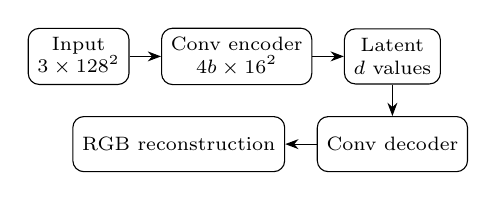
\begin{tikzpicture}[node distance=4mm, every node/.style={draw,rounded corners,font=\scriptsize,align=center,minimum height=7mm},>=Stealth]
\node (x) {Input\\$3\times128^2$};
\node (e) [right=of x] {Conv encoder\\$4b\times16^2$};
\node (z) [right=of e] {Latent\\$d$ values};
\node (d) [below=of z] {Conv decoder};
\node (y) [left=of d] {RGB reconstruction};
\draw[->] (x)--(e);\draw[->] (e)--(z);\draw[->] (z)--(d);\draw[->] (d)--(y);
\end{tikzpicture}\caption{Task 1 compressed restoration path. Tasks 2 and 3 reuse this expert architecture.}\end{figure}

\section{Task 2: Classification and Hard Routing}
A four-stage convolutional classifier uses global average pooling, dropout,
and a four-logit linear head. Multiclass cross entropy supervises the corruption
label generated by the data loader. Three independently optimized autoencoders
learn salt, blur, and occlusion restoration. A shared architecture search scores
the average validation objective across all three specialists.
\begin{equation}
r=\arg\max_k C(\tilde{x})_k,\quad
\hat{x}=\begin{cases}\tilde{x},&r=0,\\A_r(\tilde{x}),&r\ne0.\end{cases}
\end{equation}
Oracle routing selects the branch using the true manifest label; predicted
routing uses classifier argmax. Comparing these modes isolates the contribution
of routing mistakes. Clean oracle inputs have an exact identity bypass; a
misclassified clean input can be unnecessarily altered in predicted mode.
Accuracy, macro precision/recall/F1, per-class metrics, a normalized confusion
matrix, and individual routing failures are included after evaluation.

\begin{figure}[!ht]\centering
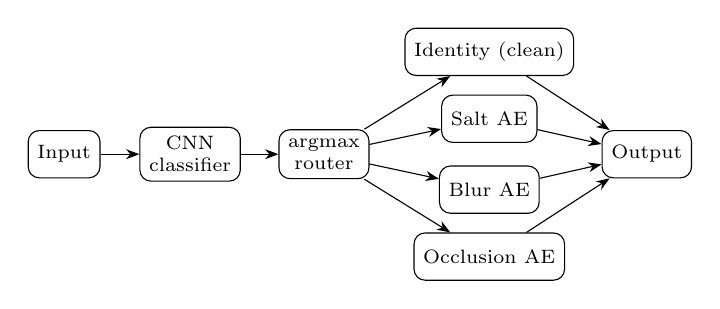
\begin{tikzpicture}[every node/.style={draw,rounded corners,font=\scriptsize,align=center,minimum height=6mm},>=Stealth]
\node (x) at (0.3,0) {Input};
\node (c) at (1.9,0) {CNN\\classifier};
\node (r) at (3.6,0) {argmax\\router};
\node (e0) at (5.7,1.3) {Identity (clean)};
\node (e1) at (5.7,0.45) {Salt AE};
\node (e2) at (5.7,-0.45) {Blur AE};
\node (e3) at (5.7,-1.3) {Occlusion AE};
\node (y) at (7.7,0) {Output};
\draw[->] (x)--(c);\draw[->] (c)--(r);
\foreach \i in {0,1,2,3} {\draw[->] (r)--(e\i);\draw[->] (e\i)--(y);}
\end{tikzpicture}\caption{Task 2 hard routing: the classifier selects exactly one branch; clean inputs bypass restoration.}\end{figure}

\section{Task 3: Joint Soft Mixture}
The gate is initialized from the trained classifier and the three experts from
Task 2. An initial two-epoch warm-up trains only the gate with experts frozen;
the experts are then unfrozen and the complete system is fine-tuned jointly.
Both stages use one Adam learning rate, searched in $[10^{-5},3\times10^{-4}]$
(selected $2.7\times10^{-4}$, below the classifier's $7.9\times10^{-4}$ and
slightly below the specialists' $3\times10^{-4}$); it is not reduced a second
time at unfreezing.
\begin{align}
w&=\mathrm{softmax}(G(\tilde{x})/\tau),\\
\hat{x}&=w_0\tilde{x}+\sum_{k=1}^{3}w_k A_k(\tilde{x}),\\
\mathcal{L}_{joint}&=\alpha\mathcal{L}_1+(1-\alpha)(1-\mathrm{SSIM})\nonumber\\
&\quad+\lambda_{cls}\mathcal{L}_{CE}+\lambda_{bal}\sum_{k=0}^{3}(\bar{w}_k-1/4)^2.
\end{align}
The balance target assumes balanced training batches. A temperature above one
softens weights; a lower value sharpens them. Mean weights per condition and
severity, distributed and dominant examples, and branches receiving under 1\%
mean weight are reported. The inference graph evaluates all branches, so it
does not inherit sparse-compute speed advantages.
\begin{figure}[!ht]\centering
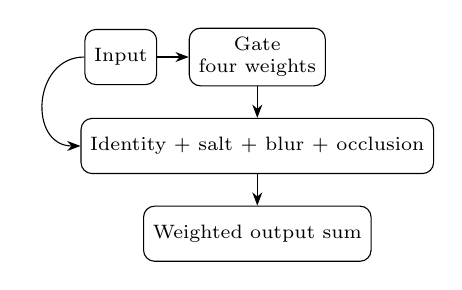
\begin{tikzpicture}[node distance=4mm, every node/.style={draw,rounded corners,font=\scriptsize,align=center,minimum height=7mm},>=Stealth]
\node (x) {Input};\node (g) [right=of x] {Gate\\four weights};
\node (b) [below=of g] {Identity + salt + blur + occlusion};
\node (s) [below=of b] {Weighted output sum};
\draw[->] (x)--(g);\draw[->] (x.west) to[out=180,in=180,looseness=1.5] (b.west);\draw[->] (g)--(b);\draw[->] (b)--(s);
\end{tikzpicture}\caption{Soft routing; hard routing instead uses argmax and executes one selected branch.}\end{figure}

\section{Task 4: Style-Conditioned Face-to-Sketch GAN}
A five-level U-Net downsamples from 128 to 4 pixels and upsamples through
skip-connected decoding stages. A learned style embedding is spatially
broadcast and concatenated with the photograph. The discriminator separately
embeds the same style, concatenating it with photograph and sketch. Its three
stride-two convolutional stages followed by a stride-one logit convolution
produce local real/fake predictions. The refined generator uses BatchNorm with tracked inference statistics in encoder and intermediate decoder stages, learned convolution and PixelShuffle upsampling, and phase-matched ICNR initialization \cite{shi,aitken}. The discriminator normalizes its second and third downsampling stages. Dropout is applied to early decoder stages.
\begin{align}
\mathcal{L}_D&=\tfrac12[\mathrm{BCE}(D(x,y,s),1)+\mathrm{BCE}(D(x,G(x,s),s),0)],\\
\mathcal{L}_G&=\mathrm{BCE}(D(x,G(x,s),s),1)+\lambda_1\|G(x,s)-y\|_1.
\end{align}
Discriminator real/fake losses and generator adversarial/reconstruction losses
are logged separately. The same fixed validation photographs are saved every
five epochs. Only the generator is deployed. Cross-style outputs on one photo
are qualitative evidence; paired metrics apply to its annotated style only.

\begin{figure}[!ht]\centering
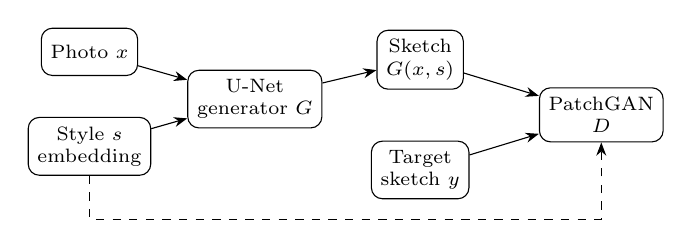
\begin{tikzpicture}[every node/.style={draw,rounded corners,font=\scriptsize,align=center,minimum height=6mm},>=Stealth]
\node (p) at (0.4,1.0) {Photo $x$};
\node (s) at (0.4,-0.2) {Style $s$\\embedding};
\node (g) at (2.5,0.4) {U-Net\\generator $G$};
\node (y) at (4.6,0.9) {Sketch\\$G(x,s)$};
\node (t) at (4.6,-0.5) {Target\\sketch $y$};
\node (d) at (6.9,0.2) {PatchGAN\\$D$};
\draw[->] (p)--(g);\draw[->] (s)--(g);\draw[->] (g)--(y);
\draw[->] (y)--(d);\draw[->] (t)--(d);
\draw[->,dashed] (s.south) -- ++(0,-0.55) -| (d.south);
\end{tikzpicture}\caption{Task 4 conditional GAN. The style embedding enters both $G$ and $D$ (dashed); $D$ outputs a map of local real/fake scores.}\end{figure}


\section{Hyperparameter Search and Training}
Optuna TPE samples configurations and median pruning stops unpromising
individual-model trials \cite{optuna,optunapaper}. Short trials use 3 epochs, 40 training batches and 40 validation batches for the new restoration and GAN studies; the historical classifier study retains its original budget; each study records its actual
budget and trial outcomes. The shared specialist study evaluates all three
specialists and does not use intermediate pruning. Selected restoration configurations are trained from scratch on the full training split; the classifier is retained and the refined GAN is independently tuned and trained from scratch. Adam \cite{adam} is used; GAN
optimizers use $(\beta_1,\beta_2)=(0.5,0.999)$. CUDA runs use mixed precision;
gradient norms are clipped to five. Checkpoints include optimizer, scaler,
random state, epoch, configuration, and data hashes for recovery.

\begin{table}[!ht]\centering\caption{Search spaces (selected model generation)}\scriptsize
\begin{tabular}{p{.25\linewidth}p{.65\linewidth}}\toprule Study & Searched parameters\\\midrule
Universal & LR $10^{-4}$--$.0005$; batch 16/32/64; base 16/24/32; latent 2048/4096/8192; dropout 0--.08; $\alpha$ .6--.95\\
Classifier & LR $10^{-4}$--$.003$; batch 16/32/64; base 8/16/24; dropout 0--.3; weight decay $10^{-6}$--$10^{-3}$\\
Specialists & Shared LR, batch, base, latent, dropout, $\alpha$ as universal\\
Soft & LR $10^{-5}$--$.0003$; batch 16/32/64; $\tau$ .5--2; $\lambda_{cls}$ .02--.3; $\lambda_{bal}$ .001--.1; $\alpha$ .6--.95\\
GAN & Generator LR $10^{-4}$--$.0005$; discriminator LR $.0001$--$.001$; batch 16/32/64; base 16/24/32; dropout 0--.08; embedding 4/8/16; $\lambda_1$ 50--150\\\bottomrule
\end{tabular}\end{table}
MLflow records configurations, losses, validation metrics and sample artifacts
\cite{mlflow}. Exploratory pilots used a free Colab T4 without mounting Google Drive. After its free GPU quota was reached and temporary new weights were lost, improvement searches and final training ran on the laptop CPU with persistent local checkpoints, optimizer/RNG state and SQLite databases. Earlier downloaded models and records were preserved separately. Limited studies cannot support a claim of
globally optimal architectures.

\section{Evaluation and Results}
PSNR is computed per image with range one and then averaged. SSIM and L1 use
the same preprocessing for every system. Clean identity PSNR is capped at
100 dB through the numeric floor on mean-squared error. Each pet test image has
ten deterministic input conditions (36,690 inputs in a full evaluation).
Per-image CSVs preserve routing labels, errors and scores. Subset evaluations
are explicitly labelled and must not be represented as full test results.
\statusnote{Measured test results; complete evaluation.}

\subsection{Task 1: Universal model}

\begin{table}[!ht]\centering\caption{Task 1: Universal model}\scriptsize

\begin{tabular}{llrrrr}\toprule Condition & Severity & $n$ & L1 & PSNR & SSIM\\\midrule

clean & clean & 3669 & 0.0338 & 26.61 & 0.8216\\

salt & low & 3669 & 0.0371 & 25.76 & 0.7695\\

salt & medium & 3669 & 0.0416 & 24.75 & 0.7206\\

salt & high & 3669 & 0.0478 & 23.58 & 0.6656\\

blur & low & 3669 & 0.0333 & 26.69 & 0.8212\\

blur & medium & 3669 & 0.0359 & 25.88 & 0.7827\\

blur & high & 3669 & 0.0436 & 24.11 & 0.6881\\

occlusion & low & 3669 & 0.0427 & 23.62 & 0.7602\\

occlusion & medium & 3669 & 0.0513 & 21.85 & 0.7042\\

occlusion & high & 3669 & 0.0659 & 19.80 & 0.6173\\

\bottomrule\end{tabular}\end{table}

Mean per-input PSNR is 24.26 dB; the corrupted-input baseline is 27.31 dB. Clean identity inputs influence these averages, so condition-specific rows should guide interpretation.

Salt: PSNR changes relative to leaving the corrupted input unchanged are +5.62, +8.88, +10.44 dB at low/medium/high severity; the fixed reconstruction objective improves in 3 of 3 severity groups.

Blur: PSNR changes relative to leaving the corrupted input unchanged are -5.65, -0.89, -0.24 dB at low/medium/high severity; the fixed reconstruction objective improves in 0 of 3 severity groups.

Occlusion: PSNR changes relative to leaving the corrupted input unchanged are +7.01, +8.62, +9.12 dB at low/medium/high severity; the fixed reconstruction objective improves in 2 of 3 severity groups.

On clean inputs, L1 is 0.03376, SSIM is 0.82163, and the fixed objective is 0.06268. The identity reference has no reconstruction error; any clean-image degradation is therefore a limitation.

\evidencefigure{universal_representative_1.png}{Task 1: Universal model: representative examples 1-4. Columns: clean target, input, output, absolute error.}

\evidencefigure{universal_representative_2.png}{Task 1: Universal model: representative examples 5-8. Columns: clean target, input, output, absolute error.}

\evidencefigure{universal_representative_3.png}{Task 1: Universal model: representative examples 9-12. Columns: clean target, input, output, absolute error.}

\evidencefigure{universal_failures.png}{Task 1: Universal model: four lowest-PSNR examples with distinct source images.}

Failure 1: Egyptian\_Mau\_60, occlusion at high severity, PSNR 8.72 dB and SSIM 0.1795. 
Large masks hide most of the cat/background; smooth guessed colors fail to recover the scene.

Failure 2: Ragdoll\_78, occlusion at high severity, PSNR 8.80 dB and SSIM 0.4455. 
The mask crosses the face and body; fur detail is lost and the filled region remains blurry.

Failure 3: chihuahua\_84, occlusion at medium severity, PSNR 10.02 dB and SSIM 0.4394. 
Background occlusion is filled by a broad smooth band instead of the original textured scene.

Failure 4: shiba\_inu\_95, occlusion at high severity, PSNR 10.83 dB and SSIM 0.4572. 
Masks across the head and muzzle produce inaccurate face colors and blurred contours.

\subsection{Task 2: Oracle routing}

\begin{table}[!ht]\centering\caption{Task 2: Oracle routing}\scriptsize

\begin{tabular}{llrrrr}\toprule Condition & Severity & $n$ & L1 & PSNR & SSIM\\\midrule

clean & clean & 3669 & 0.0000 & 100.00 & 1.0000\\

salt & low & 3669 & 0.0343 & 26.40 & 0.8163\\

salt & medium & 3669 & 0.0354 & 26.10 & 0.8012\\

salt & high & 3669 & 0.0381 & 25.46 & 0.7720\\

blur & low & 3669 & 0.0338 & 26.65 & 0.8299\\

blur & medium & 3669 & 0.0334 & 26.63 & 0.8198\\

blur & high & 3669 & 0.0405 & 24.78 & 0.7234\\

occlusion & low & 3669 & 0.0438 & 23.56 & 0.7654\\

occlusion & medium & 3669 & 0.0509 & 21.92 & 0.7182\\

occlusion & high & 3669 & 0.0638 & 19.81 & 0.6402\\

\bottomrule\end{tabular}\end{table}

Mean per-input PSNR is 32.13 dB; the corrupted-input baseline is 27.31 dB. Clean identity inputs influence these averages, so condition-specific rows should guide interpretation.

Salt: PSNR changes relative to leaving the corrupted input unchanged are +6.26, +10.23, +12.32 dB at low/medium/high severity; the fixed reconstruction objective improves in 3 of 3 severity groups.

Blur: PSNR changes relative to leaving the corrupted input unchanged are -5.69, -0.15, +0.42 dB at low/medium/high severity; the fixed reconstruction objective improves in 2 of 3 severity groups.

Occlusion: PSNR changes relative to leaving the corrupted input unchanged are +6.95, +8.69, +9.13 dB at low/medium/high severity; the fixed reconstruction objective improves in 2 of 3 severity groups.

On clean inputs, L1 is 0.00000, SSIM is 1.00000, and the fixed objective is 0.00000. The identity reference has no reconstruction error; any clean-image degradation is therefore a limitation.

\subsection{Task 2: Predicted routing}

\begin{table}[!ht]\centering\caption{Task 2: Predicted routing}\scriptsize

\begin{tabular}{llrrrr}\toprule Condition & Severity & $n$ & L1 & PSNR & SSIM\\\midrule

clean & clean & 3669 & 0.0055 & 87.60 & 0.9714\\

salt & low & 3669 & 0.0355 & 26.27 & 0.8129\\

salt & medium & 3669 & 0.0354 & 26.10 & 0.8012\\

salt & high & 3669 & 0.0381 & 25.46 & 0.7720\\

blur & low & 3669 & 0.0318 & 27.08 & 0.8415\\

blur & medium & 3669 & 0.0335 & 26.61 & 0.8188\\

blur & high & 3669 & 0.0406 & 24.76 & 0.7227\\

occlusion & low & 3669 & 0.0438 & 23.51 & 0.7662\\

occlusion & medium & 3669 & 0.0509 & 21.92 & 0.7182\\

occlusion & high & 3669 & 0.0638 & 19.81 & 0.6402\\

\bottomrule\end{tabular}\end{table}

Mean per-input PSNR is 30.91 dB; the corrupted-input baseline is 27.31 dB. Clean identity inputs influence these averages, so condition-specific rows should guide interpretation.

Salt: PSNR changes relative to leaving the corrupted input unchanged are +6.14, +10.23, +12.32 dB at low/medium/high severity; the fixed reconstruction objective improves in 3 of 3 severity groups.

Blur: PSNR changes relative to leaving the corrupted input unchanged are -5.25, -0.17, +0.41 dB at low/medium/high severity; the fixed reconstruction objective improves in 1 of 3 severity groups.

Occlusion: PSNR changes relative to leaving the corrupted input unchanged are +6.90, +8.69, +9.13 dB at low/medium/high severity; the fixed reconstruction objective improves in 2 of 3 severity groups.

On clean inputs, L1 is 0.00552, SSIM is 0.97136, and the fixed objective is 0.01014. The identity reference has no reconstruction error; any clean-image degradation is therefore a limitation.

\evidencefigure{predicted_routing_representative_1.png}{Task 2: Predicted routing: representative examples 1-4. Columns: clean target, input, output, absolute error.}

\evidencefigure{predicted_routing_representative_2.png}{Task 2: Predicted routing: representative examples 5-8. Columns: clean target, input, output, absolute error.}

\evidencefigure{predicted_routing_representative_3.png}{Task 2: Predicted routing: representative examples 9-12. Columns: clean target, input, output, absolute error.}

\evidencefigure{predicted_routing_failures.png}{Task 2: Predicted routing: four lowest-PSNR examples with distinct source images.}

Failure 1: Egyptian\_Mau\_60, salt at low severity, PSNR 7.10 dB and SSIM 0.2550. 
The classifier selected occlusion, differing from the true salt condition. 
Salt noise is misclassified as occlusion on a dark background; the wrong expert produces severe smoothing and false background colors.

Failure 2: Sphynx\_23, salt at low severity, PSNR 8.28 dB and SSIM 0.3397. 
The classifier selected occlusion, differing from the true salt condition. 
Salt noise is misclassified as occlusion on a dark background; the wrong expert produces severe smoothing and false background colors.

Failure 3: Egyptian\_Mau\_97, salt at low severity, PSNR 8.65 dB and SSIM 0.3181. 
The classifier selected occlusion, differing from the true salt condition. 
Salt noise is misclassified as occlusion on a dark background; the wrong expert produces severe smoothing and false background colors.

Failure 4: Egyptian\_Mau\_63, salt at low severity, PSNR 8.81 dB and SSIM 0.3762. 
The classifier selected occlusion, differing from the true salt condition. 
Salt noise is misclassified as occlusion on a dark background; the wrong expert produces severe smoothing and false background colors.

\subsection{Task 3: Soft mixture}

\begin{table}[!ht]\centering\caption{Task 3: Soft mixture}\scriptsize

\begin{tabular}{llrrrr}\toprule Condition & Severity & $n$ & L1 & PSNR & SSIM\\\midrule

clean & clean & 3669 & 0.0033 & 50.65 & 0.9948\\

salt & low & 3669 & 0.0343 & 26.50 & 0.8294\\

salt & medium & 3669 & 0.0359 & 26.05 & 0.8120\\

salt & high & 3669 & 0.0375 & 25.64 & 0.7887\\

blur & low & 3669 & 0.0225 & 29.86 & 0.9091\\

blur & medium & 3669 & 0.0317 & 27.16 & 0.8395\\

blur & high & 3669 & 0.0388 & 25.13 & 0.7344\\

occlusion & low & 3669 & 0.0402 & 20.32 & 0.8600\\

occlusion & medium & 3669 & 0.0506 & 21.61 & 0.7445\\

occlusion & high & 3669 & 0.0667 & 19.32 & 0.6418\\

\bottomrule\end{tabular}\end{table}

Mean per-input PSNR is 27.23 dB; the corrupted-input baseline is 27.31 dB. Clean identity inputs influence these averages, so condition-specific rows should guide interpretation.

Salt: PSNR changes relative to leaving the corrupted input unchanged are +6.37, +10.18, +12.50 dB at low/medium/high severity; the fixed reconstruction objective improves in 3 of 3 severity groups.

Blur: PSNR changes relative to leaving the corrupted input unchanged are -2.48, +0.38, +0.78 dB at low/medium/high severity; the fixed reconstruction objective improves in 2 of 3 severity groups.

Occlusion: PSNR changes relative to leaving the corrupted input unchanged are +3.72, +8.39, +8.64 dB at low/medium/high severity; the fixed reconstruction objective improves in 3 of 3 severity groups.

On clean inputs, L1 is 0.00330, SSIM is 0.99477, and the fixed objective is 0.00369. The identity reference has no reconstruction error; any clean-image degradation is therefore a limitation.

\evidencefigure{soft_representative_1.png}{Task 3: Soft mixture: representative examples 1-4. Columns: clean target, input, output, absolute error.}

\evidencefigure{soft_representative_2.png}{Task 3: Soft mixture: representative examples 5-8. Columns: clean target, input, output, absolute error.}

\evidencefigure{soft_representative_3.png}{Task 3: Soft mixture: representative examples 9-12. Columns: clean target, input, output, absolute error.}

\evidencefigure{soft_failures.png}{Task 3: Soft mixture: four lowest-PSNR examples with distinct source images.}

Failure 1: Egyptian\_Mau\_60, occlusion at medium severity, PSNR 11.63 dB and SSIM 0.4195. 
The mixture fills a masked dark background with incorrect smooth colors.

Failure 2: german\_shorthaired\_96, occlusion at low severity, PSNR 11.88 dB and SSIM 0.8767. 
A visible speckled face is partly retained rather than cleaned; the mixture still loses some detail.

Failure 3: staffordshire\_bull\_terrier\_92, occlusion at high severity, PSNR 12.02 dB and SSIM 0.7187. 
Large masks across the face/body produce a blurred, inaccurate animal reconstruction.

Failure 4: boxer\_91, occlusion at high severity, PSNR 12.32 dB and SSIM 0.4844. 
The large foreground mask destroys body/chair detail; the mixture substitutes smooth approximate colors.

\subsection{Corruption classifier}

Overall accuracy is 0.9685. Macro precision, recall and F1 are 0.9552, 0.9452 and 0.9499.

\begin{table}[!ht]\centering\caption{Per-class classifier results}\scriptsize\begin{tabular}{lrrrr}\toprule Class & Precision & Recall & F1 & $n$\\\midrule

clean & 0.8923 & 0.8288 & 0.8594 & 3669\\

salt & 0.9918 & 0.9973 & 0.9945 & 11007\\

blur & 0.9576 & 0.9590 & 0.9583 & 11007\\

occlusion & 0.9793 & 0.9956 & 0.9874 & 11007\\

\bottomrule\end{tabular}\end{table}

\evidencefigure{confusion.png}{Normalized confusion matrix; each row is a true class. Off-diagonal entries identify routing mistakes.}

\evidencefigure{routing_error_cases.png}{Hard-routing examples with an incorrect classifier prediction. Targets and errors expose the restoration consequence.}

Egyptian\_Mau\_60: true salt (low), predicted occlusion; predicted-routing PSNR 7.10 dB versus oracle 19.99 dB (difference -12.89 dB). 
Sphynx\_23: true salt (low), predicted occlusion; predicted-routing PSNR 8.28 dB versus oracle 28.56 dB (difference -20.28 dB). 
Egyptian\_Mau\_97: true salt (low), predicted occlusion; predicted-routing PSNR 8.65 dB versus oracle 25.07 dB (difference -16.43 dB). 
Egyptian\_Mau\_63: true salt (low), predicted occlusion; predicted-routing PSNR 8.81 dB versus oracle 25.32 dB (difference -16.51 dB). 
A wrong label changes the selected branch, but its numerical effect can be positive or negative because the specialists are imperfect; classification correctness alone does not establish restoration quality.

\subsection{Expert weight analysis}

\begin{table}[!ht]\centering\caption{Mean soft branch weights}\scriptsize\begin{tabular}{llrrrr}\toprule Class & Severity & Clean & Salt & Blur & Mask\\\midrule

clean & clean & 0.911 & 0.016 & 0.029 & 0.043\\

salt & low & 0.044 & 0.953 & 0.000 & 0.003\\

salt & medium & 0.000 & 1.000 & 0.000 & 0.000\\

salt & high & 0.000 & 1.000 & 0.000 & 0.000\\

blur & low & 0.558 & 0.000 & 0.407 & 0.035\\

blur & medium & 0.291 & 0.000 & 0.690 & 0.019\\

blur & high & 0.294 & 0.000 & 0.687 & 0.019\\

occlusion & low & 0.594 & 0.009 & 0.006 & 0.391\\

occlusion & medium & 0.112 & 0.001 & 0.001 & 0.886\\

occlusion & high & 0.004 & 0.000 & 0.000 & 0.996\\

\bottomrule\end{tabular}\end{table}

\evidencefigure{routing_heatmap.png}{Mean expert contribution by true condition and severity. Concentration in unrelated rows suggests imbalance.}

Branches below 1\% global mean contribution: none.

Examples with dominant weights: 
Bombay\_76 (clean=0.000, salt=1.000, blur=0.000, occlusion=0.000); 
Egyptian\_Mau\_60 (clean=0.000, salt=1.000, blur=0.000, occlusion=0.000); 
these examples demonstrate gate concentration, not automatically improved restoration.

Examples with distributed weights: 
shiba\_inu\_9 (clean=0.322, salt=0.000, blur=0.341, occlusion=0.337); 
pug\_74 (clean=0.357, salt=0.349, blur=0.000, occlusion=0.294); 
these examples demonstrate gate concentration, not automatically improved restoration.

\subsection{Task 4: Face-to-sketch results}

\begin{table}[!ht]\centering\caption{Paired sketch reconstruction by style}\begin{tabular}{lrrrr}\toprule Style & $n$ & L1 & PSNR & SSIM\\\midrule

1 & 619 & 0.0876 & 16.58 & 0.5006\\

2 & 381 & 0.1707 & 11.53 & 0.3654\\

3 & 46 & 0.0701 & 18.19 & 0.5725\\

\bottomrule\end{tabular}\end{table}

\evidencefigure{face_representative_1.png}{Paired sketch examples 1-4: target, photograph, output and absolute error.}

\evidencefigure{face_representative_2.png}{Paired sketch examples 5-8: target, photograph, output and absolute error.}

\evidencefigure{face_representative_3.png}{Paired sketch examples 9-12: target, photograph, output and absolute error.}

\evidencefigure{style_comparison.png}{The same photograph under all three style conditions. Only its annotated style has a paired ground truth.}

\evidencefigure{face_failures.png}{Four lowest-PSNR paired sketch reconstructions, with distinct source photographs.}

Sketch failure 1: photo1\_image1600, style 1, PSNR 7.11 dB and SSIM 0.2531. 
Dense hair strokes and dark shading are missing; the generated face is overly pale and smooth.

Sketch failure 2: photo1\_image1599, style 1, PSNR 7.20 dB and SSIM 0.2569. 
Hair and facial contours are underdrawn compared with the dense reference sketch.

Sketch failure 3: photo1\_image0837, style 2, PSNR 7.57 dB and SSIM 0.1889. 
The overall head shape is present, but textured hair/shading and fine feature lines are absent.

Sketch failure 4: photo1\_image1034, style 2, PSNR 7.59 dB and SSIM 0.1537. 
The output face is pale and smooth, missing dark hair strokes and precise facial contours.

\subsection{Observed failure modes and interpretation}

Earlier dense and small spatial bottlenecks produced collapsed or blurry reconstructions. A larger 16-by-16 compressed representation with local residual refinement was investigated. A learning-rate 0.001 pilot saturated and was rejected. The subsequent lower-rate pilot reached validation objective 0.14389, compared with 0.24516 for the previous selected model. This motivated a separate Optuna study and longer training, with all selection based on validation.

\begin{table}[!ht]\centering\caption{Validation-led architecture pilots}\scriptsize\begin{tabular}{lrrrr}\toprule Pilot & Epoch & Objective & PSNR & SSIM\\\midrule

Low LR & 14 & 0.2074 & 16.56 & 0.4336\\

BatchNorm & 5 & 0.2012 & 16.67 & 0.4465\\

Learned upsampling & 10 & 0.1439 & 20.28 & 0.5786\\

\bottomrule\end{tabular}\end{table}

These sequential pilots are exploratory, not controlled single-factor ablations: capacity, normalization, learning rate and upsampling differ. Their saved images and complete validation histories are retained. The selected learned-upsampling pilot used standard initialization; fresh final models use phase-matched ICNR initialization to address periodic artifacts, without guaranteeing their removal.

\begin{table}[!ht]\centering\caption{Complete validation comparison, lower objective is better}\scriptsize\begin{tabular}{lrrr}\toprule System & Previous & Candidate & Change (\%)\\\midrule

universal & 0.2452 & 0.0853 & -65.2\\

oracle\_routing & 0.2217 & 0.0704 & -68.3\\

predicted\_routing & 0.2232 & 0.0710 & -68.2\\

soft & 0.1325 & 0.0642 & -51.5\\

gan & 0.1898 & 0.1853 & -2.4\\

\bottomrule\end{tabular}\end{table}

Both model sets use the same complete validation inputs and fixed objective $0.8\,L_1+0.2(1-\mathrm{SSIM})$. Numerical improvements must be considered with the per-condition changes and saved images; a lower aggregate score does not establish improvement on every input.

The corruption classifier is retained from the preceding validation-selected run, while a normalized GAN with learned upsampling is tuned in a new study and trained from scratch. Restoration and routing quality are judged using condition-specific metrics and failure grids, not successful API execution alone.

Fresh CPU training from saved validation evidence after free Colab GPU quota; pilot weights were lost. The saved pilot measurements survived, but its weights did not. The improved models were trained afresh on the laptop CPU, while the retained classifier and exploratory pilots used the earlier free GPU runs. Local and Colab data manifests match after newline normalization.

The fixed final improvement schedule was universal=24 epochs, specialists=20 epochs, soft=12 epochs, gan=60 epochs. This deadline-aware budget was chosen before inspecting the final candidate test results.

\subsection{Completed search and training records}

universal: 2 completed trials, 1 pruned trials; best trial 0, validation objective 0.14329. The short-trial budget and complete search space are preserved in the study JSON.

\evidencefigure{optuna_universal.png}{Completed validation trial objectives for universal. These limited searches are not exhaustive.}

classifier: 3 completed trials, 1 pruned trials; best trial 3, validation objective 0.32709. The short-trial budget and complete search space are preserved in the study JSON.

\evidencefigure{optuna_classifier.png}{Completed validation trial objectives for classifier. These limited searches are not exhaustive.}

specialists: 3 completed trials, 0 pruned trials; best trial 0, validation objective 0.13232. The short-trial budget and complete search space are preserved in the study JSON.

\evidencefigure{optuna_specialists.png}{Completed validation trial objectives for specialists. These limited searches are not exhaustive.}

soft: 2 completed trials, 1 pruned trials; best trial 1, validation objective 0.06718. The short-trial budget and complete search space are preserved in the study JSON.

\evidencefigure{optuna_soft.png}{Completed validation trial objectives for soft. These limited searches are not exhaustive.}

gan: 2 completed trials, 1 pruned trials; best trial 0, validation objective 0.21116. The short-trial budget and complete search space are preserved in the study JSON.

\evidencefigure{optuna_gan.png}{Completed validation trial objectives for gan. These limited searches are not exhaustive.}

Selected universal checkpoint: epoch 22. Configuration: base=24, latent=8192, dropout=0.0, batch\_size=32, lr=0.0003, weight\_decay=1e-05, alpha=0.8, temperature=1.0, classification\_weight=0.1, balance\_weight=0.01, embedding=8, discriminator\_lr=0.0002, l1\_weight=100.0, detail=True, detail\_bn=True, detail\_shuffle=True.

\evidencefigure{curve_universal.png}{Recorded training and validation objectives for universal; differing objectives may have different scales.}

Selected classifier checkpoint: epoch 10. Configuration: base=24, latent=128, dropout=0.2896896099223678, batch\_size=32, lr=0.0007896186801026692, weight\_decay=0.0002661901888489054, alpha=0.8, temperature=1, classification\_weight=0.1, balance\_weight=0.01, embedding=8, discriminator\_lr=0.0002, l1\_weight=100.

\evidencefigure{curve_classifier.png}{Recorded training and validation objectives for classifier; differing objectives may have different scales.}

Selected salt checkpoint: epoch 20. Configuration: base=24, latent=8192, dropout=0.0, batch\_size=32, lr=0.0003, weight\_decay=1e-05, alpha=0.8, temperature=1.0, classification\_weight=0.1, balance\_weight=0.01, embedding=8, discriminator\_lr=0.0002, l1\_weight=100.0, detail=True, detail\_bn=True, detail\_shuffle=True.

\evidencefigure{curve_salt.png}{Recorded training and validation objectives for salt; differing objectives may have different scales.}

Selected blur checkpoint: epoch 18. Configuration: base=24, latent=8192, dropout=0.0, batch\_size=32, lr=0.0003, weight\_decay=1e-05, alpha=0.8, temperature=1.0, classification\_weight=0.1, balance\_weight=0.01, embedding=8, discriminator\_lr=0.0002, l1\_weight=100.0, detail=True, detail\_bn=True, detail\_shuffle=True.

\evidencefigure{curve_blur.png}{Recorded training and validation objectives for blur; differing objectives may have different scales.}

Selected occlusion checkpoint: epoch 18. Configuration: base=24, latent=8192, dropout=0.0, batch\_size=32, lr=0.0003, weight\_decay=1e-05, alpha=0.8, temperature=1.0, classification\_weight=0.1, balance\_weight=0.01, embedding=8, discriminator\_lr=0.0002, l1\_weight=100.0, detail=True, detail\_bn=True, detail\_shuffle=True.

\evidencefigure{curve_occlusion.png}{Recorded training and validation objectives for occlusion; differing objectives may have different scales.}

Selected soft checkpoint: epoch 11. Configuration: base=16, latent=128, dropout=0.1, batch\_size=32, lr=0.00027081608642499667, weight\_decay=1e-05, alpha=0.6641915784487018, temperature=1.7486639612006325, classification\_weight=0.035543498097189236, balance\_weight=0.0023102018878452934, embedding=8, discriminator\_lr=0.0002, l1\_weight=100.0.

\evidencefigure{curve_soft.png}{Recorded training and validation objectives for soft; differing objectives may have different scales.}

Selected gan checkpoint: epoch 12. Configuration: base=24, latent=128, dropout=0.05, batch\_size=32, lr=0.0002, weight\_decay=1e-05, alpha=0.8, temperature=1.0, classification\_weight=0.1, balance\_weight=0.01, embedding=16, discriminator\_lr=0.0002, l1\_weight=100.0, gan\_refined=True.

\evidencefigure{curve_gan.png}{Recorded training and validation objectives for gan; differing objectives may have different scales.}


\section{Discussion of Results}\label{sec:discussion}
\begin{table}[!ht]\centering\caption{Mean test PSNR (dB) / SSIM per condition, averaged over severities (clean PSNR is capped at 100 dB)}\label{tab:means}\scriptsize

\setlength{\tabcolsep}{3pt}\begin{tabular}{lcccc}\toprule System & Clean & Salt & Blur & Occlusion\\\midrule

Input (unrestored) & 100.0/1.000 & 16.4/0.382 & 27.8/0.814 & 13.5/0.702\\

Universal & 26.6/0.822 & 24.7/0.719 & 25.6/0.764 & 21.8/0.694\\

Oracle routing & 100.0/1.000 & 26.0/0.796 & 26.0/0.791 & 21.8/0.708\\

Predicted routing & 87.6/0.971 & 25.9/0.795 & 26.2/0.794 & 21.7/0.708\\

Soft mixture & 50.7/0.995 & 26.1/0.810 & 27.4/0.828 & 20.4/0.749\\

\bottomrule\end{tabular}\end{table}

Table~\ref{tab:means} condenses the per-severity tables above. The paragraphs below interpret them; causal explanations are marked as hypotheses where no ablation was run.

\paragraph{Salt-and-pepper noise.} This is the clearest success. Relative to leaving the noisy input unchanged, mean PSNR rises by +8.3 dB (universal), +9.6 dB (oracle specialist), +9.6 dB (predicted routing) and +9.7 dB (soft mixture); specialist SSIM is 0.796 against 0.382 for the input. The dedicated specialist beats the universal model by 0.6 dB at low severity and 1.9 dB at high severity, consistent with the hypothesis that a single network sharing capacity across conditions does worse as noise grows. This is a comparison under our training budget, not a proof that specialisation is always superior.

\paragraph{Occlusion.} PSNR rises by +8.3 dB for oracle routing because black holes are filled with plausible colours. SSIM is mixed: at low severity the specialist SSIM (0.765) is below the unrestored input (0.857), because the autoencoder re-synthesises every pixel, including those the input already had exactly, whereas at high severity SSIM improves from 0.528 to 0.640. The failure grids show large masks across faces filled with smooth guessed colour, not recovered texture.

\paragraph{Blur.} This is the weakest condition. Mean PSNR change relative to the unrestored blurred input is -2.3 dB (universal), -1.8 dB (oracle), -1.7 dB (predicted) and -0.4 dB (soft). Oracle routing changes PSNR by -5.7, -0.1, +0.4 dB at low, medium and high severity, so restoration helps only at the highest severity and then by under one dB. A likely explanation is the reconstruction ceiling of the compressed latent: even on clean inputs the universal model reaches only 26.6 dB, while the blur specialist reaches 26.6 dB at low severity, where the unrestored input already scores 32.3 dB. Passing a lightly blurred image through the bottleneck is therefore likely to lower fidelity. No larger-latent ablation was run, so this is a hypothesis consistent with the data, not a demonstrated cause.

\paragraph{Clean inputs.} The universal model alters clean images (PSNR 26.6 dB, SSIM 0.822), a cost that hard routing and the soft mixture largely avoid through the identity branch: predicted routing keeps SSIM at 0.971, and the soft mixture at 0.995 because the gate gives the identity branch a mean weight of 91.1\% on clean images.

\paragraph{Classifier and hard routing.} The classifier reaches 96.8\% accuracy. Its errors concentrate in the clean class: clean recall is 0.829 and 12.5\% of clean images are labelled blur. This is expected because low-severity blur (a $3\times3$ kernel with $\sigma=0.7$) barely differs from a clean photograph; salt-and-pepper is almost always recognised (recall 0.997). 
Predicted routing differs from oracle routing by only -0.12 to +0.44 dB per condition on average, because few corrupted images are misrouted (for example 3.1\% of blurred images are labelled clean, where bypassing the specialist can even help low-severity blur). Misrouting can nevertheless be severe: 
the four worst predicted-routing cases are salt-and-pepper images sent to the occlusion expert (PSNR 7.1--8.8 dB against 20.0--28.6 dB with the correct expert); the saved failure analysis notes dark backgrounds.

\paragraph{Soft gate.} For salt-and-pepper the gate is nearly one-hot (salt expert weight 0.953 at low severity and at least 0.9996 at medium and high severity). For blur and occlusion at low severity it shares weight with the identity branch (identity weights 0.56 and 0.59). This explains why the soft model beats the specialists on low-severity blur (29.9 versus 26.6 dB) yet fills less of the mask at low-severity occlusion (20.3 versus 23.6 dB PSNR, 0.860 versus 0.765 SSIM). No branch contributes under 1\% of the global mean weight, so no expert is inactive, and no unrelated expert exceeds a mean weight of 0.043, so none dominates unrelated inputs. 
The price is compute: the soft graph evaluates all four branches, with single-request CPU inference of 25.4 ms against 12.4 ms for hard routing and 12.9 ms for the universal model.

\paragraph{Face-to-sketch.} Mean SSIM over the 1,046 test pairs is 0.455; style 2 ($n=381$) is weakest at 11.5 dB PSNR, while style 3 has only 46 test pairs, so its score is noisy. The generated sketches reproduce head pose and outline but are pale and smooth, without the hatching of the references (see the failure analysis). 
Discriminator real and fake losses stay between 0.36 and 0.83, so neither network overwhelms the other. The validation objective is lowest at epoch 12 (0.185) and is 0.201 at epoch 60: longer adversarial training did not improve the L1/SSIM-based objective, so the epoch-12 checkpoint is deployed. 
Plausible causes are the small generator, only 899 training pairs at $128\times128$, and the weight-100 L1 term favouring averaged outputs; none was isolated by an experiment.

\paragraph{How the evidence shaped the design.} Validation pilots decided the architecture. The validation objective of the first dense-latent model was 0.322; an $8\times8$ spatial latent reached 0.281, a $16\times16$ latent with local residual blocks 0.207, and the final design (8,192-value latent, BatchNorm, PixelShuffle upsampling) 0.144 in its pilot and 0.085 after full training. These runs differ in budget, so the sequence indicates direction, not a controlled ablation. The remaining weaknesses above, blur and sketch detail, are the points where additional capacity, a sharper loss or a longer GPU schedule would be tried next.


\section{Application Architecture and Deployment}
The React/Tailwind interface provides four workspaces in one application.
FastAPI validates JPEG, PNG and WebP uploads, rejects files over 10 MB and
oversized decoded images, applies optional reproducible corruption, and runs
ONNX Runtime CPU inference. It returns input/output PNGs, route probabilities
or soft weights, and inference latency. Runtime corruption makes the clean
reference available for an error map; an arbitrary uploaded corrupted image
does not provide an assumed ground truth.
\begin{table}[!ht]\centering\caption{Backend endpoints}\scriptsize
\begin{tabular}{>{\raggedright\arraybackslash}p{.42\linewidth}>{\raggedright\arraybackslash}p{.46\linewidth}}\toprule Endpoint & Purpose\\\midrule
GET \texttt{/api/health} & Per-model and per-workspace readiness\\
GET \texttt{/api/samples} & Clean sample images\\
GET \texttt{/api/experiments} & Test metrics and MLflow run records\\
POST \texttt{/api/corrupt} & Reproducible corruption preview\\
POST \texttt{/api/universal-restoration} & Task 1 inference\\
POST \texttt{/api/hard-routing} & Task 2: probabilities, expert, output\\
POST \texttt{/api/soft-mixture} & Task 3: four weights, output\\
POST \texttt{/api/face-to-sketch} & Task 4: photo and style to sketch\\\bottomrule
\end{tabular}\end{table}

The frontend is served by Nginx and proxies API requests to the backend.
Docker Compose starts both containers using
\texttt{docker compose up --build}; the browser URL is
\url{http://localhost:8080}. Model and result directories are mounted read-only.
Session initialization is excluded from inference timing. Missing models,
synthetic test checkpoints and failed checksum verification produce a clear
unavailable-model state rather than substitute output.

ONNX export checks random, black and white inputs for batches of one and two,
including all three GAN styles. Acceptance uses absolute tolerance $10^{-4}$
and relative tolerance $10^{-3}$ for every output. Actual maximum deviations
are stored in the deployment manifest. The complete soft inference pipeline is
one graph; the classifier and specialists are separate graphs for hard routing.

\begin{figure}[!ht]\centering
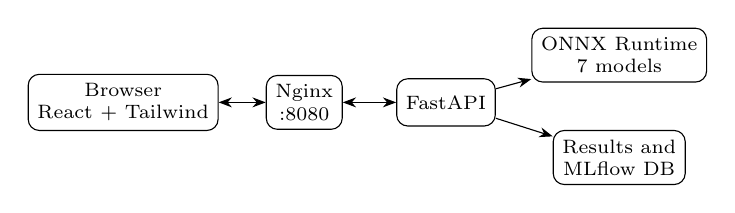
\begin{tikzpicture}[every node/.style={draw,rounded corners,font=\scriptsize,align=center,minimum height=6mm},>=Stealth]
\node (b) at (0.9,0) {Browser\\React + Tailwind};
\node (n) at (3.2,0) {Nginx\\:8080};
\node (f) at (5.0,0) {FastAPI};
\node (o) at (7.2,0.6) {ONNX Runtime\\7 models};
\node (m) at (7.2,-0.7) {Results and\\MLflow DB};
\draw[<->] (b)--(n);\draw[<->] (n)--(f);\draw[->] (f)--(o);\draw[->] (f)--(m);
\end{tikzpicture}\caption{Deployment: two Docker Compose services; model and result files are mounted read-only into the backend.}\end{figure}
\evidencefigure{app-experiments.jpg}{Application with imported trained ONNX models: app-experiments}

\evidencefigure{app-hard.jpg}{Application with imported trained ONNX models: app-hard}

\evidencefigure{app-sketch.jpg}{Application with imported trained ONNX models: app-sketch}

\evidencefigure{app-soft.jpg}{Application with imported trained ONNX models: app-soft}

\evidencefigure{app-tracking.jpg}{Application with imported trained ONNX models: app-tracking}

\evidencefigure{app-universal.jpg}{Application with imported trained ONNX models: app-universal}

Local verification passed all seven model checksums and finite-output checks, all four API workspaces, and all three sketch styles using CPUExecutionProvider. Measured sample-request inference times ranged from 10.66 to 25.43 ms. These are single-request checks, not a throughput benchmark. The universal black-versus-white output difference was 9.79e-01. This confirms input sensitivity for these two controls, not restoration quality.\par

\evidencefigure{stitch-original.png}{Original Google Stitch universal-workspace design. Decorative metrics and classes in this mockup are not experiment results.}

Stitch's HTML and PNG exports are retained in the repository (\texttt{docs/stitch-evidence}). The implemented interface was reconciled with this design: dark navigation rail with the four workspaces, input panel, result panel, error and experiment views, and a green palette. Mock-up metrics and class names that correspond to no implemented function (for example the A100 latency badge and the ViT parameter counts) were omitted from the working application.\par

\statusnote{Docker Compose was built and executed with a Linux Docker engine. HTTP tests passed for all four workspaces and all three sketch styles at localhost:8080.}
\subsection{Links}

Repository: \url{https://github.com/Abdullah73/genai-assignment-1}.\par

Original Stitch design: \url{https://stitch.withgoogle.com/projects/16111510614845497849}.\par


\section{Limitations and Conclusion}
The main limitations are the following. (1) The compact bottleneck discards
fine texture, which appears to cap reconstruction near the level reached on clean inputs,
so blur restoration does not exceed the uncorrected input on average.
(2) Optuna searches used short trials (three epochs, 40 batches) and few trials,
so the selected configurations are the best of a small search, not a global
optimum; in three studies the best trial was the seeded starting configuration.
(3) The classifier confuses clean and low-severity blurred inputs, and the soft
gate shares that ambiguity. (4) The sketch generator produces smooth, pale
sketches without hatching; style~3 has only 46 test pairs, so its scores are
noisy. (5) Single-corruption training does not establish reliable
mixed-corruption restoration, and disjoint-band masks do not cover all real
occlusion geometries. (6) Inference is $128\times128$ on CPU; larger uploads are
resized. (7) Final training used a CPU after free GPU quota was exhausted, which
limited schedule length. (8) The soft mixture keeps its warm-up learning rate
after unfreezing the experts instead of lowering it, as the assignment suggests;
the effect of such a drop was not tested.
Future work should enlarge the latent for blur, add a sharpening or perceptual
loss, run longer GAN schedules with more Optuna trials on a GPU, and evaluate
mixed corruptions.
The measured results above characterize the selected compact models under the recorded training budget; broader claims require further experiments.

\appendices
\section{AI Use and Verification}
\begin{table}[!ht]\centering\caption{AI tools used, purpose and verification}\scriptsize
\renewcommand{\arraystretch}{1.12}\begin{tabular}{>{\raggedright\arraybackslash}p{.16\linewidth}>{\raggedright\arraybackslash}p{.34\linewidth}>{\raggedright\arraybackslash}p{.32\linewidth}}\toprule
Tool & Used for & How outputs were checked\\\midrule
OpenAI Codex & Reading the assignment, finding sources, drafting models, training and evaluation code, FastAPI/React code, Colab notebook, tests, first report draft & 20 automated tests (corruptions, balanced batches, paired augmentation, SSIM, bottleneck, gradients through all mixture branches, style conditioning, upload validation, resume, ONNX), validation grids, ONNX-vs-PyTorch comparison, Docker runs\\
Anthropic Claude (Claude Code) & Final audit of the repository against the assignment, report revision (protocol, discussion, limitations), documentation and repository packaging & Numbers in the discussion are computed from the saved result files by the report script; documents compared with files; tests re-run\\
Google Stitch & Original interface design (exports retained in the repository) & Controls compared with implemented functions; decorative mock-up metrics omitted\\\bottomrule
\end{tabular}\end{table}
A soft-mixture dropout-mode mismatch found by ONNX consistency testing was
corrected. Synthetic-data tests verify mechanics only; dataset performance
comes from saved real checkpoints evaluated on deterministic manifests.
The student remains responsible for understanding and explaining every
component.

\begin{thebibliography}{99}
\bibitem{vincent} P. Vincent et al., ``Stacked denoising autoencoders: Learning useful representations in a deep network with a local denoising criterion,'' JMLR, vol. 11, pp. 3371--3408, 2010.
\bibitem{wang} Z. Wang, A. C. Bovik, H. R. Sheikh, and E. P. Simoncelli, ``Image quality assessment: From error visibility to structural similarity,'' IEEE TIP, vol. 13, no. 4, pp. 600--612, 2004.
\bibitem{shazeer} N. Shazeer et al., ``Outrageously large neural networks: The sparsely-gated mixture-of-experts layer,'' arXiv:1701.06538, 2017.
\bibitem{isola} P. Isola, J.-Y. Zhu, T. Zhou, and A. A. Efros, ``Image-to-image translation with conditional adversarial networks,'' CVPR, pp. 1125--1134, 2017.
\bibitem{pets} O. M. Parkhi et al., ``Cats and dogs,'' CVPR, 2012. Dataset: \url{https://www.robots.ox.ac.uk/~vgg/data/pets/}.
\bibitem{fs2k} FS2K dataset, official release, 2021. \url{https://github.com/DengPingFan/FS2K}.
\bibitem{optuna} Optuna documentation, efficient optimization algorithms. \url{https://optuna.readthedocs.io/en/stable/tutorial/10_key_features/003_efficient_optimization_algorithms.html}.
\bibitem{mlflow} MLflow documentation, experiment tracking. \url{https://mlflow.org/docs/latest/ml/tracking/}.
\bibitem{shi} W. Shi et al., ``Real-time single image and video super-resolution using an efficient sub-pixel convolutional neural network,'' CVPR, 2016. \url{https://arxiv.org/abs/1609.05158}.
\bibitem{aitken} A. Aitken et al., ``Checkerboard artifact free sub-pixel convolution: A note on sub-pixel convolution, resize convolution and convolution resize,'' arXiv:1707.02937, 2017.
\bibitem{hinton} G. E. Hinton and R. R. Salakhutdinov, ``Reducing the dimensionality of data with neural networks,'' Science, vol. 313, no. 5786, pp. 504--507, 2006.
\bibitem{dncnn} K. Zhang, W. Zuo, Y. Chen, D. Meng, and L. Zhang, ``Beyond a Gaussian denoiser: Residual learning of deep CNN for image denoising,'' IEEE TIP, vol. 26, no. 7, pp. 3142--3155, 2017.
\bibitem{unet} O. Ronneberger, P. Fischer, and T. Brox, ``U-Net: Convolutional networks for biomedical image segmentation,'' MICCAI, 2015.
\bibitem{jacobs} R. A. Jacobs, M. I. Jordan, S. J. Nowlan, and G. E. Hinton, ``Adaptive mixtures of local experts,'' Neural Computation, vol. 3, no. 1, pp. 79--87, 1991.
\bibitem{switch} W. Fedus, B. Zoph, and N. Shazeer, ``Switch Transformers: Scaling to trillion parameter models with simple and efficient sparsity,'' JMLR, vol. 23, no. 120, 2022.
\bibitem{gan} I. Goodfellow et al., ``Generative adversarial nets,'' NeurIPS, 2014.
\bibitem{cgan} M. Mirza and S. Osindero, ``Conditional generative adversarial nets,'' arXiv:1411.1784, 2014.
\bibitem{fs2kpaper} D.-P. Fan et al., ``Facial-sketch synthesis: A new challenge,'' Machine Intelligence Research, vol. 19, no. 4, pp. 257--287, 2022.
\bibitem{adam} D. P. Kingma and J. Ba, ``Adam: A method for stochastic optimization,'' ICLR, 2015.
\bibitem{optunapaper} T. Akiba, S. Sano, T. Yanase, T. Ohta, and M. Koyama, ``Optuna: A next-generation hyperparameter optimization framework,'' KDD, 2019.
\bibitem{batchnorm} S. Ioffe and C. Szegedy, ``Batch normalization: Accelerating deep network training by reducing internal covariate shift,'' ICML, 2015.
\end{thebibliography}
\end{document}
